\documentclass[10pt]{article}

\usepackage[T2A]{fontenc}
\usepackage[utf8]{inputenc}
\usepackage[english, russian]{babel}
\usepackage{amssymb}
\usepackage{url}

\usepackage{fancyvrb}
\usepackage{color}
\usepackage{pdfpages}
\usepackage{caption}
\usepackage{subcaption}

\usepackage{listings}
\usepackage{algpseudocode}
\usepackage{algorithmicx}

\usepackage{cmap}
\usepackage{natbib}
\setlength{\bibsep}{0.2pt}

\newtheorem{definition}{Определение}

\algnewcommand\algorithmicswitch{\textbf{switch}}
\algnewcommand\algorithmiccase{\textbf{case}}
\algnewcommand\algorithmicassert{\texttt{assert}}
\algnewcommand\Assert[1]{\State \algorithmicassert(#1)}

\algdef{SE}[SWITCH]{Switch}{EndSwitch}[1]{\algorithmicswitch\ #1\ \algorithmicdo}{\algorithmicend\ \algorithmicswitch}
\algdef{SE}[CASE]{Case}{EndCase}[1]{\algorithmiccase\ #1}{\algorithmicend\ \algorithmiccase}

\algtext*{EndSwitch}
\algtext*{EndCase}
\algtext*{EndWhile}
\algtext*{EndIf}
\algtext*{EndFor}
\algtext*{EndFunction}
\algtext*{EndProcedure}

\title{Динамически формируемый код: синтаксический анализ \\ контекстно-свободной аппроксимации}
\author{
    Дмитрий Ковалев, Семён Григорьев \\
    \textit{Санкт-Петербургский государственный университет,} \\
    \textit{Россия, 199034, Санкт-Петербург, Университетская наб. 7/9} \\
    \url{dmitry.kovalev-m@ya.ru}, \url{semen.grigorev@jetbrains.com} }
\date{}

\begin{document}

\maketitle

%%
%% The abstract is a short summary of the work to be presented in the
%% article.
\begin{abstract}
В последнее время наблюдается рост интереса к решению задач, связанных с контекстно-свободными запросами на графах.
Критически важной становится потребность в измерении производительности алгоритмов решающих подобные задачи.
Тем не менее разработка наборов контрольных данных и стандартизированные процедуры оценки отстают, что препятствует продвижению вперед в этой области.
Чтобы решить эти проблемы мы представляем коллекцию CFPQ\_Data, в которой собраны наиболее популярные графы для проведения экспериментального анализа алгоритмов решающих задачи контекстно-свободных запросов на графах.
Коллекция состоит из более чем 40 графов разного размера.
Также мы предоставляем загрузчики данных и реализации наиболее популярных алгоритмов на основе Python, а также стандарт проведения экспериментов и базовых показателей работы алгоритма.
Здесь мы даем обзор собранной коллекции, стандартизированных процедур исследования и проводим базовые эксперименты.
Все наборы данных доступны на сайте \href{https://github.com/JetBrains-Research/CFPQ_Data}{https://github.com/JetBrains-Research/CFPQ\_Data}.
Проведенные эксперименты полностью воспроизводимы из кода, доступного на сайте \href{https://github.com/JetBrains-Research/CFPQ_PyAlgo}{https://github.com/JetBrains-Research/CFPQ\_PyAlgo}.
\end{abstract}

\section{Introduction}

Scalable high-performance graph analysis is an actual challenge.
There is a big number of ways to attack this challenge~\cite{Coimbra2021} and the first promising idea is to utilize general-purpose graphic processing units (GPGPU).
Such existing solutions, as CuSha~\cite{10.1145/2600212.2600227} and Gunrock~\cite{7967137} show that utilization of GPUs can improve the performance of graph analysis, moreover it is shown that solutions may be scaled to multi-GPU systems.
But low flexibility and high complexity of API are problems of these solutions.

The second promising thing which provides a user-friendly API for high-performance graph analysis algorithms creation is a GraphBLAS API~\cite{7761646} which provides linear algebra based building blocks to create graph analysis algorithms.
The idea of GraphBLAS is based on a well-known fact that linear algebra operations can be efficiently implemented on parallel hardware.
Along with that, a graph can be natively represented using matrices: adjacency matrix, incidence matrix, etc.
While reference CPU-based implementation of GraphBLAS, SuiteSparse:GraphBLAS~\cite{10.1145/3322125}, demonstrates good performance in real-world tasks, GPU-based implementation is challenging.

One of the challenges in this way is that real data are often sparse, thus underlying matrices and vectors are also sparse, and, as a result, classical dense data structures and respective algorithms are inefficient. 
So, it is necessary to use advanced data structures and procedures to implement sparse linear algebra, but the efficient implementation of them on GPU is hard due to the irregularity of workload and data access patterns.
Though such well-known libraries as cuSPARSE show that sparse linear algebra operations can be efficiently implemented for GPGPU, it is not so trivial to implement GraphBLAS on GPGPU. 
First of all, it requires \textit{generic} sparse linear algebra, thus it is impossible just to reuse existing libraries which are almost all specified for operations over floats.
The second problem is specific optimizations, such as masking fusion, which can not be natively implemented on top of existing kernels.
Nevertheless, there is a number of implementations of GraphBLAS on GPGPU, such as GraphBLAST~\cite{yang2019graphblast}, GBTL~\cite{7529957}, which show that GPGPUs utilization can improve the performance of GraphBLAS-based graph analysis solutions.
But these solutions are not portable because they are based on Nvidia Cuda stack.
Moreover, the scalability problem is not solved: all these solutions support only single-GPU, not multi-GPU computations.

To provide portable GPU implementation of GraphBLAS API we developed a \textit{SPLA} library\footnote{Source code available at: \url{https://github.com/JetBrains-Research/spla}}.
This library utilizes OpenCL for GPGPU computing to be portable across devices of different vendors.
Moreover, it is initially designed to utilize multiple GPGPUs to be scalable.
To sum up, the contribution of this work is the following.
\begin{itemize}
    \item Design of portable GPU GraphBLAS implementation proposed. The design involves the utilization of multiple GPUS. Additionally, the proposed design is aimed to simplify library tuning and wrappers for different high-level platforms and languages creation. 
    \item Subset of GraphBLAS API, including such operations as masking, matrix-matrix multiplication, matrix-matrix e-wise addition, is implemented. The current implementation is limited by COO and CSR matrix representation format and uses basic algorithms for some operations, but work in progress and more data formats will be supported and advanced algorithms will be implemented in the future.
    \item Preliminary evaluation on such algorithms as breadth-first search (BFS) and triangles counting (TC), and real-world graphs shows portability across different vendors and promising performance: for some problems Spla is comparable with GraphBLAST. Surprisingly, for some problems, the proposed solution on embedded Intel graphic card shows better performance than SuiteSparse:GraphBLAS on the respective CPU. At the same time, the evaluation shows that further optimization is required.
\end{itemize} 
\section{Обзор}

Для того чтобы упростить ход рассуждений, касающихся контекстно-свободных грамматик, в данной работе используется понятие \textit{рекурсивного автомата} --- абстракции, позволяющей задавать произвольную КС-грамматику.
Ее описание приводится в первом параграфе обзора. 
Второй параграф посвящен вопросу о разрешимости задачи синтаксического анализа контекстно-свободного представления данных и его связи с фундаментальными проблемами теории формальных языков.

Предлагаемый в данной работе алгоритм основан на алгоритме синтаксического анализа регулярных множеств, который, в свою очередь, явлется модификацией алгоритма обобщенного синтаксического анализа Generalized LL. 
Об этих алгоритмах, а также о проекте, в рамках которого проведена разработка предложенного решения, также будет рассказано в обзоре.

\subsection{Рекурсивные автоматы и КС-грамматики}
Введем понятие рекурсивного автомата, которое потребуется для дальнейшего изложения

\begin{defn}
	Рекурсивный автомат R --- это пятерка $(\Sigma, Q, \delta, q_0, q_f)$, где $\Sigma$ --- конечное множество терминальных символов, $Q$ --- конечное множество состояний автомата, $\delta : Q \times (\Sigma \cup Q) \rightarrow 2^Q$ --- функция переходов, $q_0 \in Q$ --- начальное состояние, $q_f$ --- конечное состояние. 
\end{defn}

Можно заметить, что данное определение практически идентично определению стандартного конечного автомата. 
Единственное отличие состоит в том, что метками на ребрах рекурсивного автомата могут как терминальные символы (терминальные переходы), так и состояния (нетерминальные переходы).
Класс рекурсивных автоматов обладает такой же выразительностью, как и контекстно-свободные грамматики, т.е. позволяет описать любой контекстно-свободный язык. 
Более того, грамматика тривиальным образом может быть преобразована в рекурсивный автомат (обратное тоже верно) \cite{tellier2006ra}. 
Пример рекурсивного автомата, построенного по грамматике, можно увидеть на рисунке \ref{fig:ra_ex}.

\begin{figure}[h]
	\centering
	\begin{subfigure}[b]{0.45\textwidth}
		\centering
		$$
		\begin{array}{crcl}
		&S' & ::= & S \\
		&S  & ::= & \texttt{[ } S \texttt{ ]}\\
		&S  & ::= & \mbox{\texttt{a}}
		\end{array}
		$$
		\caption{Грамматика $G_1$}
	\end{subfigure}
	~
	\begin{subfigure}[b]{0.45\textwidth}
		\centering
		\includegraphics[width=4cm]{pictures/ra_example.pdf}
		\caption{Рекурсивный автомат для $G_1$}
	\end{subfigure}
	\caption{Преобразование между грамматикой и рекурсивным автоматом}
	\label{fig:ra_ex}
\end{figure}


\subsection{Разрешимость задачи синтаксического анализа контекстно-свободного представления}
Как было сказано ранее, задачу поиска шаблона, при условии, что и шаблон, и данные, в которых осуществляется поиск, представлены контекстно-свободными грамматиками, мы назовем синтаксическим анализом контекстно-свободного представления. 

Для доказательства предложений, сформулированных далее, будет использоваться следующая теорема \cite{Nederhof}.

\begin{theorem}[Nederhof, Satta]
	Пусть $G_1$ --- произвольная контекстно-свободная грамматика, $G_2$ --- грамматика, которая не содержит непосредственной или скрытой рекурсий. Тогда проблема проверки пустоты пересечения языков, порождаемых данными грамматиками, относится к классу PSPACE-complete.
\end{theorem}

Рассмотрим случай, когда грамматика данных задает ровно одну строку. Пусть $G_t$ --- произвольная КС-грамматика, задающая шаблоны для поиска, а $G_d$ --- КС-грамматика, которая не содержит непосредственной или скрытой рекурсий. $L(G_t)$ и $L(G_d)$ --- языки, порождаемые грамматиками, при этом $L(G_d) = \{\omega\}$, где $\omega$ --- исходные данные, к которым был применен алгоритм сжатия. 
Необходимо определить, существуют ли такие строки $\omega'$, что $\omega' \in L(G_t)$ и $\omega'$ --- подстрока $\omega$.

%т.е. $\omega' \in L_{sub}(\omega)$, где $L_{sub}(s)$ --- обозначение для языка, состоящего из всех подстрок заданной строки $s$. Отметим, что $L_{sub}$ относится к классу регулярных языков, так как множество всех подстрок конечно. 

\begin{prop}
	При выполнении описанных условий задача синтаксического анализа КС-представления разрешима.
\end{prop}

\begin{proof}
Пользуясь эквивалентностью представлений, можно записать грамматику $G_d$ в виде рекурсивного автомата $R_d$. Рассмотрим рекурсивный автомат $R_{i,\,j}$, полученный из $R_d$ путем замены стартового состояния на $i \in Q(R_d)$ и назначения терминирующего (финального, из которого не может быть совершено переходов) состояния $j \in Q(R_d)$. Такой автомат описывает грамматику, которая является представленим некоторой подстроки $\omega$. 
%В таком случае, рекурсивный автомат $R_{i,\,j}$, полученный из $R_d$ путем замены стартового и конечного состояний на $i, j \in Q(R_d)$ соответственно, описывает грамматику, которая является представленим некоторой подстроки $\omega$. 
Рассмотрев все возможные пары $i$ и $j$, получаем конечное множество грамматик, для каждой из которых необходимо проверить, содержится ли строка, порождаемая ей, в языке $L(G_t)$. 
Согласно теореме 1, такая проверка является разрешимой задачей и принадлежит к классу PSPACE-complete.
\end{proof}

Отдельно отметим, что для описанных процедур используется лишь исходный автомат, эквивалентный грамматике $G_d$. 
Условия задачи поиска шаблонов непосредственно в контекстно-свободном представлении, таким образом, выполняются. 
Верна также разрешимость более общей задачи.

\begin{prop}
	Пусть грамматика $G_d$ задает конечное множество строк $L(G_d) = \{\omega_1, \, \dots \, , \omega_n \}$. Необходимо определить, существуют ли строки $\omega'$, для которых верно: $\omega' \in L(G_t)$ и $\omega'$ --- подстрока одной из строк $\omega_i \in L(G_d)$. Данная задача разрешима и принадлежит классу PSPACE-complete.
\end{prop}

\begin{proof}
	Как и в предыдущем доказательстве, используем запись грамматики в виде рекурсивного автомата $R_d$ и рассмотрим автоматы $R_{i, j}$. В данном случае каждый из этих автоматов представляет собой грамматику, которая порождает некоторое конечное множество подстрок исходных строк из $L(G_d)$. Проверка пустоты пересечения такой грамматики с $G_t$ также соответствует условиям теоремы 1.
\end{proof}

В случае, когда грамматика $G_d$ представляет собой бесконечный регулярный язык (т.е. содержит левую и/или правую рекурсию), разрешимость задачи поиска шаблонов установить не удается. Подход, использованный ранее в доказательстве предложений, не может быть применен, так как части рекурсивного автомата, представляющего грамматику $G_d$, также могут содержать рекурсивные переходы, что выходит за рамки условия теоремы 1. Проверка разрешимости и определение класса сложности задачи проверки пустоты пересечения произвольной и регулярной КС-грамматик в настоящее время остаются открытыми проблемами \cite{Nederhof}.

%Пусть $G$ --- произвольная КС-грамматика, $M$ --- конечный автомат. Тогда задача проверки
%\begin{itemize}
%	\item включения языков ($L(M) \subseteq L(G)$) --- неразрешима
%	\item пустоты пересечения ($L(M) \cap L(G) = \emptyset$) --- разрешима (т.к. в пересечении не более чем КС-язык) за полиномиальное время \cite{Hunt}
%	\item регулярности языка $L(G)$ --- неразрешима \cite{Greibach1968}
%\end{itemize} 
%
%Если использовать представление регулярного языка $L(M)$ в виде КС-грамматики $G_r$, то задача проверки пустоты пересечения ($L(G_r) \, \cap \, L(G) = \emptyset$) становится немного интереснее: если $G_r$ 
%\begin{itemize}
%	\item нерекурсивная --- задача из PSPACE \cite{Nederhof} (точнее результата нет (я не нашел, по крайней мере))
%	\item лево- или праволинейная --- ничего не известно (см. последний абзац заключения из \cite{Nederhof})
%	\item принадлежит еще более широкому классу --- тем более ничего не известно
%\end{itemize}

%Еще немного про вложенную рекурсию и регулярность языка. Грамматика без вложенной рекурсии (NSE) порождает регулярный язык \cite{Chomsky} (обратное тоже верно, для регулярного языка можно построить NSE грамматику, т.к. праволинейная, например, --- частный случай NSE). Существует алгоритм, который позволяет проверять грамматику на наличие вложенной рекурсии за полином \cite{Anselmo}. Однако, грамматика с вложенной рекурсией тоже может порождать регулярный язык \cite{Andrei2004}, поэтому задача о проверке регулярности языка, порождаемого КС-грамматикой, остается неразрешимой. 

\subsection{GLL-алгоритм и его модификации}

Классические алгоритмы нисходящего и восходящего синтаксического анализа предполагают использование грамматики, которая является в достаточной мере однозначной. 
В противном случае, управляющие таблицы анализаторов содержат конфликты, из-за чего нельзя гарантировать корректное поведение на любых входных данных. 
Для работы с сильно неоднозначными грамматикам используются алгоритмы \textit{обобщенного синтаксического анализа}, которые позволяют рассмотреть все возможные пути разбора строки и построить соответствующие деревья вывода.
Поиск шаблонов не требует наличия деревьев вывода, поэтому в дальнейшем алгоритмы синтаксического анализа рассматриваются только как механизм, позволяющий определить принадлежность строки языку.

\subsubsection{Оригинальный GLL-алгоритм}

Generalized LL (GLL) \cite{gll} --- алгоритм, обобщающий идеи нисходящего синтаксического анализа. GLL, в отличие от стандартных LL-алгоритмов, позволяет использовать для анализа произвольную \linebreak контекстно-свободную грамматику, в том числе содержащую леворекурсивные правила. Вместе с тем, GLL наследует такие полезные свойства алгоритмов нисходящего анализа, как непосредственная связь с грамматикой и простота отладки и диагностики ошибок.

Для обработки неоднозначностей GLL разделяет стек анализатора на несколько ветвей, каждая из которых соответствует возможному пути разбора. При таком подходе необходимо компактное представление множества стеков, в качестве которого выступает Graph Structured Stack (GSS). В работе \cite{Afroozeh2015gss} была представлена модификация GSS, которая позволяет увеличить эффективность GLL-анализа. Вершины такого представления хранят в себе номер нетерминала и позицию в строке, с которой начался разбор подстроки, соответствующей ему. На ребрах хранятся позиции в грамматике (вида $X \rightarrow \alpha A \cdot \beta$), на которые необходимо вернуться после завершения разбора нетерминала. 
%При помощи GSS также решается проблема бесконечного роста стеков при обработке левой рекурсии: при попытке создать вершину, которая уже существует, в граф добавится

Основной идеей GLL является использование дескрипторов, позволяющих полностью описывать состояние анализатора в текущий момент времени.

\begin{defn}
	Дескриптор --- это тройка (L, u, i), где
	\begin{itemize}
		\setlength\itemsep{0em}
		\item L --- текущая позиция в грамматике вида $A \rightarrow \alpha \cdot \beta$
		\item u --- текущая вершина GSS
		\item i --- позиция во входном потоке 
	\end{itemize}
\end{defn}  

В процессе работы поддерживается глобальная очередь дескрипторов. В начале каждого шага исполнения алгоритм берет следующий в очереди дескриптор и производит действия в зависимости от позиции в грамматике и текущего входного символа, передвигая соответствующие указатели. 
При наличии конфликтов в грамматике алгоритм добавляет дескрипторы для каждого возможного пути анализа в конец очереди.

\subsubsection{Поддержка грамматик в EBNF}

В работе Артема Горохова \cite{Gorokhov2017ebnf} была описана модификация GLL, которая позволяет использовать грамматики, записанные в расширенной форме Бэкуса-Наура (EBNF). Грамматика такого вида трансформируется в соответствующий рекурсивный автомат, в котором затем минимизируется количество состояний. Синтаксический анализ производится без построения управляющих таблиц: алгоритм обходит рекурсивный автомат в соответствии со входным потоком символов. При обработке текущего дескриптора $(C_S, C_U, i)$, где $C_S$ --- вершина автомата (эквивалент позиции в грамматике), $C_U$ --- вершина GSS, $i$ --- позиция в строке, могут возникать следующие ситуации.

\begin{itemize}
	\item $C_S$ --- финальное состояние. Показывает, что разбор текущего нетерминала был завершен. Необходимо осуществить возврат из $C_U$ по меткам на исходящих из нее ребрах.
	\item Присутствует нетерминальный переход из $C_S$. В данном случае необходимо начать разбор указанного нетерминала $X$. Для этого в GSS должна быть создана новая вершина $(X, i)$, если она не создавалась ранее, а текущая вершина автомата изменена на стартовую для $X$.
	\item Присутствует терминальный переход из $C_S$. Необходимо сравнить терминал на ребре автомата с текущим входным символом. Если они совпадают, то осуществить переход в вершину автомата, на которую указывает ребро, и передвинуть указатель в строке.
\end{itemize}

За счет уменьшения количества состояния в автомате удается достичь прироста в производительности по сравнению со стандартным GLL-алгоритмом. 

\subsubsection{Синтаксический анализ графов}

Стандартными входными данными для алгоритмов синтаксического анализа являются линейные последовательности токенов. На основе GLL был разработан алгоритм, который позволяет производить синтаксический анализ регулярных множеств строк, представленных в виде конечного автомата (который, в свою очередь, является ориентированным графом с токенами на ребрах).

Поддержка нелинейного входа не потребовала существенных изменений в оригинальном алгоритме. Дескрипторы модифицированного алгоритма хранят номер вершины входного графа вместо позиции в строке. Также, на шаге исполнения просматривается не единственный текущий символ, а множество символов на ребрах, исходящих из текущей вершины.

Производительность данного алгоритма, как и обычного GLL, может быть увеличена при помощи представления входной грамматики в виде рекурсивного автомата. В таком случае, алгоритм будет производить обход двух автоматов --- рекурсивного и конечного. Ситуации, возникающие при обработке дексрипторов, не отличаются от описанных ранее ситуаций для линейного входа. Псевдокод данной модификации приведен в приложении.

\subsection{Проект YaccConstructor}

YaccConstructor --- исследовательский проект лаборатории языковых инструментов JetBrains на математико-механическом факультете СПбГУ, направленный на исследования в области лексического и синтаксического анализа. Проект включает в себя одноименную модульную платформу для разработки лексических и синтаксических анализаторов, содержащую большое количество компонент: язык описания грамматик YARD, преобразования над грамматиками и др. Основным языком разработки является F$\#$.

Ранее в рамках YaccConstructor были реализованы генераторы GLL-анализаторов, описание которых было приведено в данном обзоре. 

\section{Синтаксический анализ контекстно-свободной аппроксимации}

Наш алгоритм принимает на вход управляющие таблицы LL-анализа, построенные по эталонной грамматике, и GFG, который является представлением КС-грамматики --- аппроксимации множества значений выражения. 
Мы переиспользуем основные структуры данных и функции описанного ранее алгоритма анализа регулярной аппроксимации на основе GLL, расширяя данный подход для корректной обработки GFG.

Алгоритм последовательно обходит узлы GFG, производя синтаксический анализ порождаемых им строк. 
Для правильного построения таких строк, согласно определению выводимости строки в GFG-грамматике, для каждого просматриваемого пути необходимо поддерживать баланс call- и return-узлов. 
То есть, при прохождении пути алгоритм должен манипулировать дополнительным стеком (назовем его \textit{CR-стеком}). 
При достижении call-узла в стек добавляется номер return-узла, соответствующего ему; при достижении end-узла необходимо снять со стека номер return-узла и продолжить обход из него. 

Для экономии памяти мы не храним CR-стек для каждой из текущих ветвей работы алгоритма (напомним, что GLL-алгоритм может одновременно рассматривать несколько вариантов разбора строки). 
Вместо этого множество CR-стеков, по аналогии с основным стеков GLL-анализатора, представляется в виде GSS. 
Пример можно увидеть на рисунке \ref{fig:gss}. GSS позволяет хранить только одну копию общих префиксов нескольких стеков, каждый путь в нем соответствует отдельному CR-стеку.

\begin{figure}[h]
	\centering
	\includegraphics[width=6cm]{pictures/gss_cr}
	\caption{Структурированный в виде графа стек}
	\label{fig:gss}
\end{figure}

Для хранения указателя на текущую вершину стека мы добавили в дескрипторы дополнительное поле. 
Таким образом, дескриптором в нашем алгоритме называется пятерка вида $(L, u, i, w, s)$, где $i$ --- номер вершины GFG, $s$ --- указатель на вершину CR-стека в GSS, остальные поля аналогичны тем, которые представлены в дескрипторах оригинального GLL-алгоритма.

Другой особенностью работы с GFG является то, что он, в отличие от регулярной аппроксимации --- детерминированного конечного автомата, допускает возможность неоднозначного выбора пути обхода. 
Подобная ситуация возникает при наличии в исходной грамматике нескольких продукций, содержащих в левой части одинаковый нетерминал. 
Например, GFG на рисунке \ref{fig:gfg} содержит start-узел под номером 3, из которого выходит два ребра с пустой меткой (аналог $\epsilon$-переходов в конечном автомате).

Механизм дескрипторов позволяет решать проблему недетерминированного выбора пути --- для каждого из возможных вариантов создается отдельный дескриптор, который добавляется в очередь исполнения. 
Вернемся к примеру с узлом 3 на рисунке \ref{fig:gfg}. Пусть в текущий момент времени мы имеем дескриптор $(L_1, u_1, i_1, w_1, s_1)$. 
При рассмотрении ребер, выходящих из узла 3, будут созданы дескрипторы $(L_1, u_1, 4, w_1, s_1)$ и $(L_1, u_1, 5, w_1, s_1)$. Если ранее такие дескрипторы не создавались (для контроля за этим в GLL поддерживается глобальное множество создаваемых дескрипторов), они будут добавлены в очередь.

Функции \textbf{dispatcher} и \textbf{add} (проверка и добавление в очередь дескриптора) алгоритма анализа регулярной аппроксимации были незначительно изменены нами для работы с расширенными дескрипторами. 
Функция \textbf{processing} и методы для работы с основным стеком и построения SPPF переиспользованы без изменений.
Обработка start/call/exit-узлов и контроль за состоянием CR-стеков были реализованы во вспомогательной функции \textbf{closure}, псевдокод которой приведен ниже.
Она исполняется перед вызовами \textbf{dispatcher} и \textbf{processing},  %отвечающих за извлечение дескрипторов из очереди и проведение синтаксического анализа соотвественно.
производя рекурсивный обход GFG до тех пор, пока не встретит start- или scan-узел. 
При достижении start-узла создаются дескрипторы для каждого из возможных путей, и управление переходит к \textbf{dispatcher};
scan-узел обрабатывается функцией \textbf{processing} так же, как и вершина конечного автомата в оригинальном алгоритме.
%мы переиспользуем \textbf{processing} вместе с функциями построения SPPF и основного стека анализатора.

%\footnote{Отметим, что $\epsilon$-замыкание для start-узлов в общем случае не решает проблемы недетерминированного выбора, т.к. продукции, например, могут начинаться с одинакового терминального символа. Кроме того, замыкание в случае левой рекурсии приводит к появлению петель и усложняет логику работы алгоритма}

\section{Closure properties of languages with polynomial rational indices}
\label{sec:closure}
Given a context-free language $L$ with the polynomial rational index, it is interesting to find which language operations preserve this property.  Boasson et al. \cite{RatBasic} give the following useful relations for polynomial indices of two languages $L$ and $L'$.
\begin{lemma}[\cite{RatBasic}]
\label{lem:closure}
Context-free languages with polynomial rational indices are closed under intersection with a regular language, union, concatenation, the Kleene star, homomorphism and inverse homomorphism. More precisely,
\begin{itemize}
\item $\rho_{L \cup L'}(n) \le  \max{(\rho_L(n), \rho_{L'}(n))} $
\item $\rho_{LL'}(n) \le \rho_L(n) + \rho_{L'}(n)$
\item $\rho_{L^{*}}(n) \le n(\rho_L(n))$
\item $\rho_{L \cap R}(n) \le \rho_L(nm)$, where $R$ is a regular language recognised by an $m$-state automaton
\item $\rho_{h(L)}(n) \le \rho_L(n)$ and $\rho_{h^{-1}(L)}(n) < n(\rho_L(n) +1)$, where $h: \Sigma^* \rightarrow \Delta^*$ is a homomorphism
\item $\rho_{\tau(L)}(n) \le (mn + 1)\rho_L(mn)$, where $\tau$ is a rational transduction and $m$ is some integer.
\end{itemize}
\end{lemma}
 From the relations above it is easy to see that the family of context-free languages with polynomial rational indices is a full trio. Every full trio is closed under left and right quotient with regular languages, prefix, suffix, infix, and outfix \cite{GinsburgAlgebraic}. Obviously, CFLs with the polynomial rational indices languages are closed under reversal.  Next we show that context-free languages with the polynomial rational indices are closed under insertion of a regular language.
\begin{theorem}
Context-free languages with the polynomial rational indices are closed under the insertion of a regular language. 
\\Particularly, $\rho_{L_{INSERT(K)}}(n) \le (mn + 1)\rho_L(mn)$, where $m$ is the number of states in the NFA accepting $K$.
\end{theorem}
\begin{proof}
 Let $L$ be a language with the polynomial rational index over an alphabet $\Sigma$ and $K$ be a regular language over an alphabet $\Delta$, where an NFA $M(K)$ with $m$ states is an NFA accepting $K$.  Define a homomorphism $h: \Delta^*  \rightarrow \bar{\Delta}^{*}$, such that $h(a)=\bar{a}$,  $\forall a \in \Delta$. In simple words, $h$ makes all symbols from $\Delta$ ``marked''. Then, by defining a homomorphism $g$, such that $g(a) = \varepsilon$, $\forall a \in \bar{\Delta}$ ($g$ erases the symbols of $\bar{\Delta}$), one can insert an arbitrary number of symbols from $\bar{\Delta}$ into strings in $L$ using an inverse homomorphism $g^{-1}$. To obtain a string from $L_{INSERT(K)}$ it is left to intersect $g^{-1}(L)$ with a regular set $K'$ containing strings in the form $xyz$, where $x, z \subseteq \Sigma^{*}$ and $y \in h(K)$. Then ``marked'' symbols from  $\bar{\Delta}$ is unmarked by a homomorphism $\phi:  \bar{\Delta^*}  \rightarrow \Delta^{*}$, where $\phi(\bar{a}) = a$, $\forall \bar{a} \in \bar{\Delta}$. Finally, every word $w' \in L_{INSERT(K)}$ can be written as $\phi(g^{-1}(w) \cap K') = \tau(w)$, where $w \in L$ and $\tau$ is a rational transduction. By Lemma~\ref{lem:closure}, languages with the polynomial rational indices are closed under rational trunsductions, so $L_{INSERT(K)}$ has the polynomial rational index. An NFA $M(K')$ can be easily constructed from $M(K)$ and has $O(m)$ states. Then the value of the rational index $\rho_{L_{INSERT(K)}}(n) \le (mn + 1)\rho_L(mn)$.
\end{proof}



Using closure properties, it is easier to find new subclasses of context-free languages for which the CFL-reachability problem is in NC.
\begin{example}[Metalinear languages \cite{metalinear}.]
Let $G = (\Sigma, N, P, S)$ be a context-free grammar. $G$ is \textit{metalinear} if all productions of $P$ are of the following forms:
\begin{enumerate}
\item $S \rightarrow A_1A_2...A_k$, where $A_i \in N \setminus \{S\}$
\item $A \rightarrow u$, where $A \in N \setminus \{S\}$ and $u \in (\Sigma^*((N \setminus \{S\}) \cup {\varepsilon})\Sigma^*)$
\end{enumerate}


The width of a metalinear grammar is $max\{k\vert S \rightarrow A_1A_2...A_k \}$. Metalinear languages of width 1 are obviously linear languages. It is easy to see that every metalinear language is a union of concatenations of $k$ linear languages. Linear languages have polynomial rational index,  CFLs with the polynomial rational index are closed under concatenation and union, so metalinear languages have the polynomial rational index and, hence, is in NC.
\end{example}



Результатом работы алгоритма является SPPF, представляющий множество деревьев разбора всех строк, порождаемых GFG и одновременно с этим выводимых в эталонной грамматике.
\section{Conclusion and Future Work}

We present !!!

Our evaluation shows that !!!

First direction for future research is a more detailed CFPQ algorithms investigation.
We should do More evaluation on sparse matrices on GPGPUs.

Also it is nesessary to implement and evaluate solutions for graphs which is not fit in RAM.
There is a set of technics for huge matrices multiplication.
Is it possible to dopt it for CFPQ

Another direcion is a dataset improvement.
More data.
More grammars/queries.


\bibliographystyle{abbrv}
\bibliography{biblio}

\appendix

\section{\appendixname: Example of parsing and SPPF construction}\label{example}

We demonstrate the application of our algorithm by the following example. The reference grammar is shown below:

$$
\begin{array}{crcl}
(0)& start\_rule &::=& s \\
(1)& s & ::= & \mbox{\texttt{LBR }} s \mbox{\texttt{ RBR }} s\\
(2)& s & ::= &\epsilon
\end{array}
$$

The automaton for regular approximation after tokenization is shown on the Fig.~\ref{faApprox}; the 
SPPF, provided by our algorithm, is shown on the Fig.~\ref{resultSPPF}.

 \begin{figure}[!ht]
    \subfloat[Regular approximation for string-embedded code after tokenization\label{faApprox}]{%
      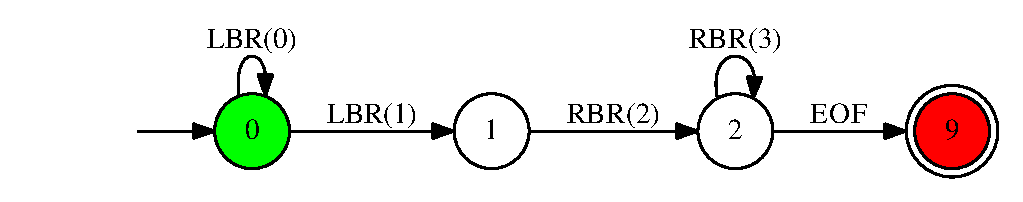
\includegraphics[scale=0.3]{dot/in3.eps}
   }  
   \hfill
    \subfloat[SPPF\label{resultSPPF}]{%
      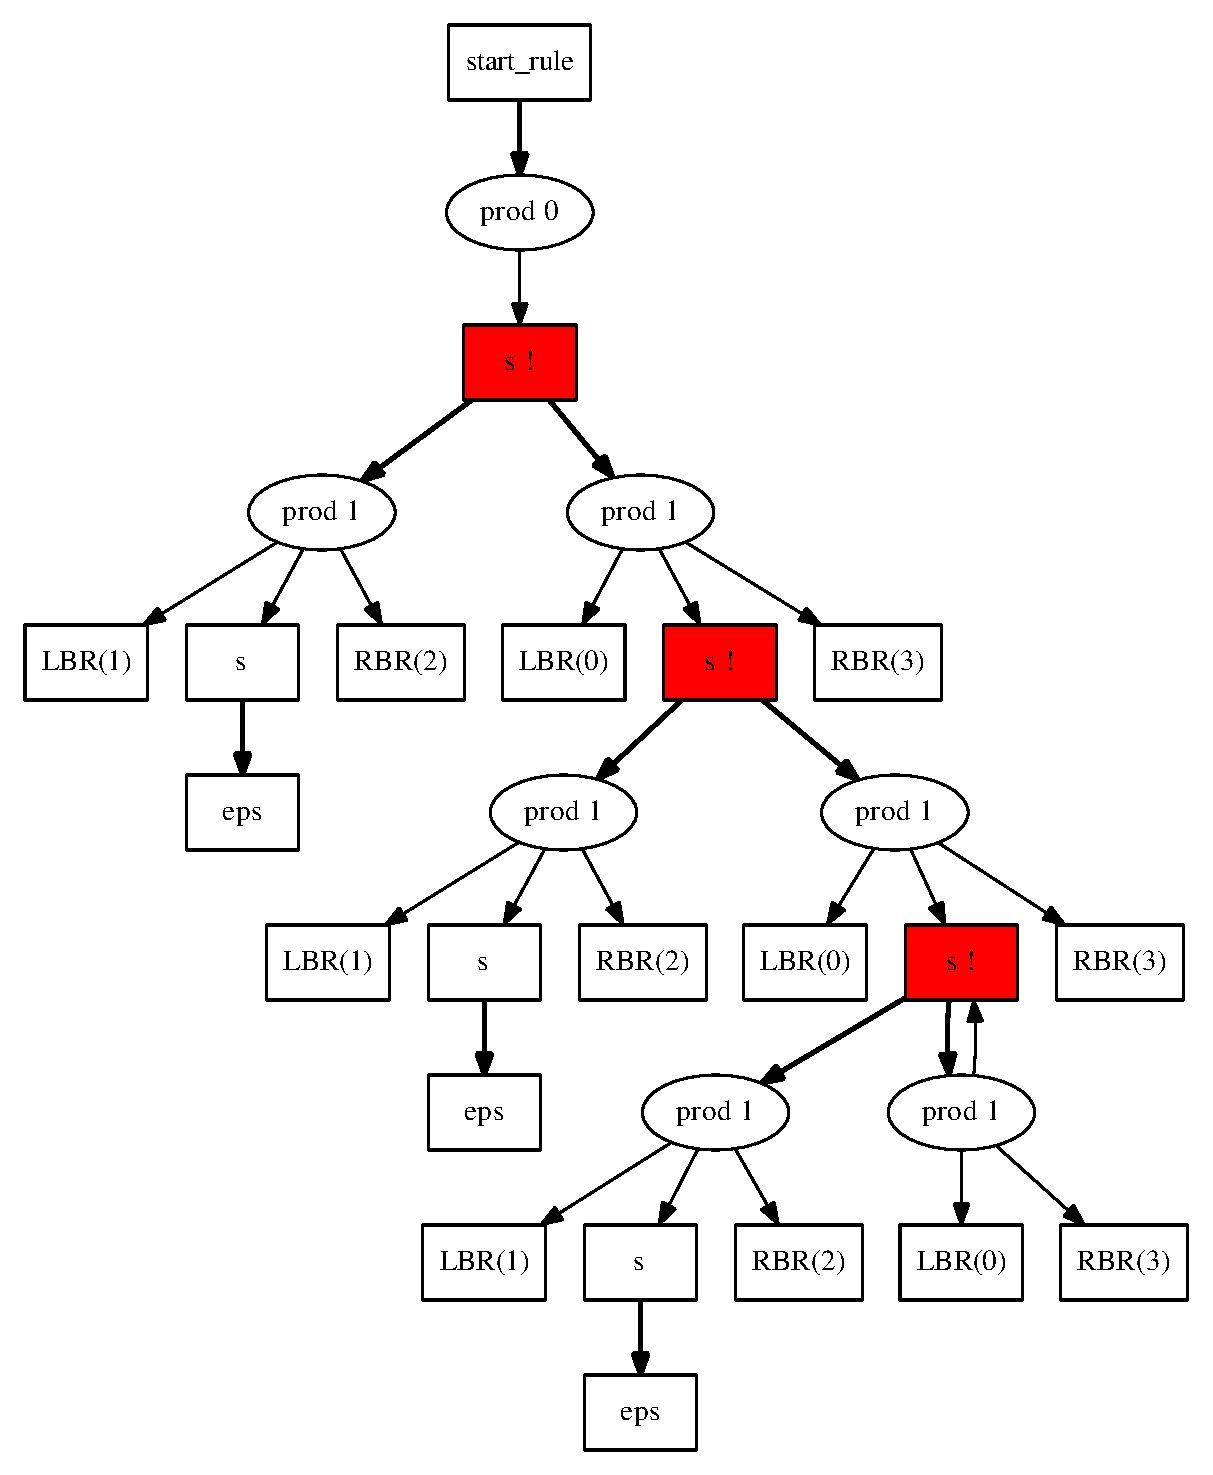
\includegraphics[scale=0.3]{dot/out3.eps}
    }
    \caption{Regular approximation and SPPF}
    \label{fig:SPPFforReg}
 \end{figure}

%\begin{figure}
%    \begin{center}
%        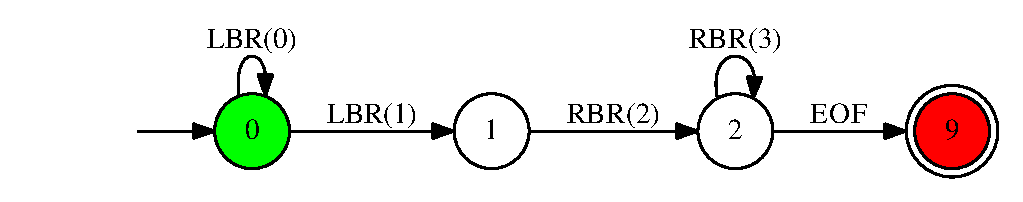
\includegraphics[scale=0.5]{dot/in3.eps}
%    \end{center}
%    \caption{$A_1$ -- input for our algorithm: regular approximation for string-embedded code after tokenization} 
%    \label{faApprox}
%\end{figure}

As it can be seen, some of the words from regular approximation do not belong to the reference language (for example, 
\verb|LBR LBR RBR|). The algorithm ignores such strings and constructs SPPF, which contains derivation trees 
for all recognized strings w.r.t. reference grammar.

%\begin{figure}
%    \begin{center}
%        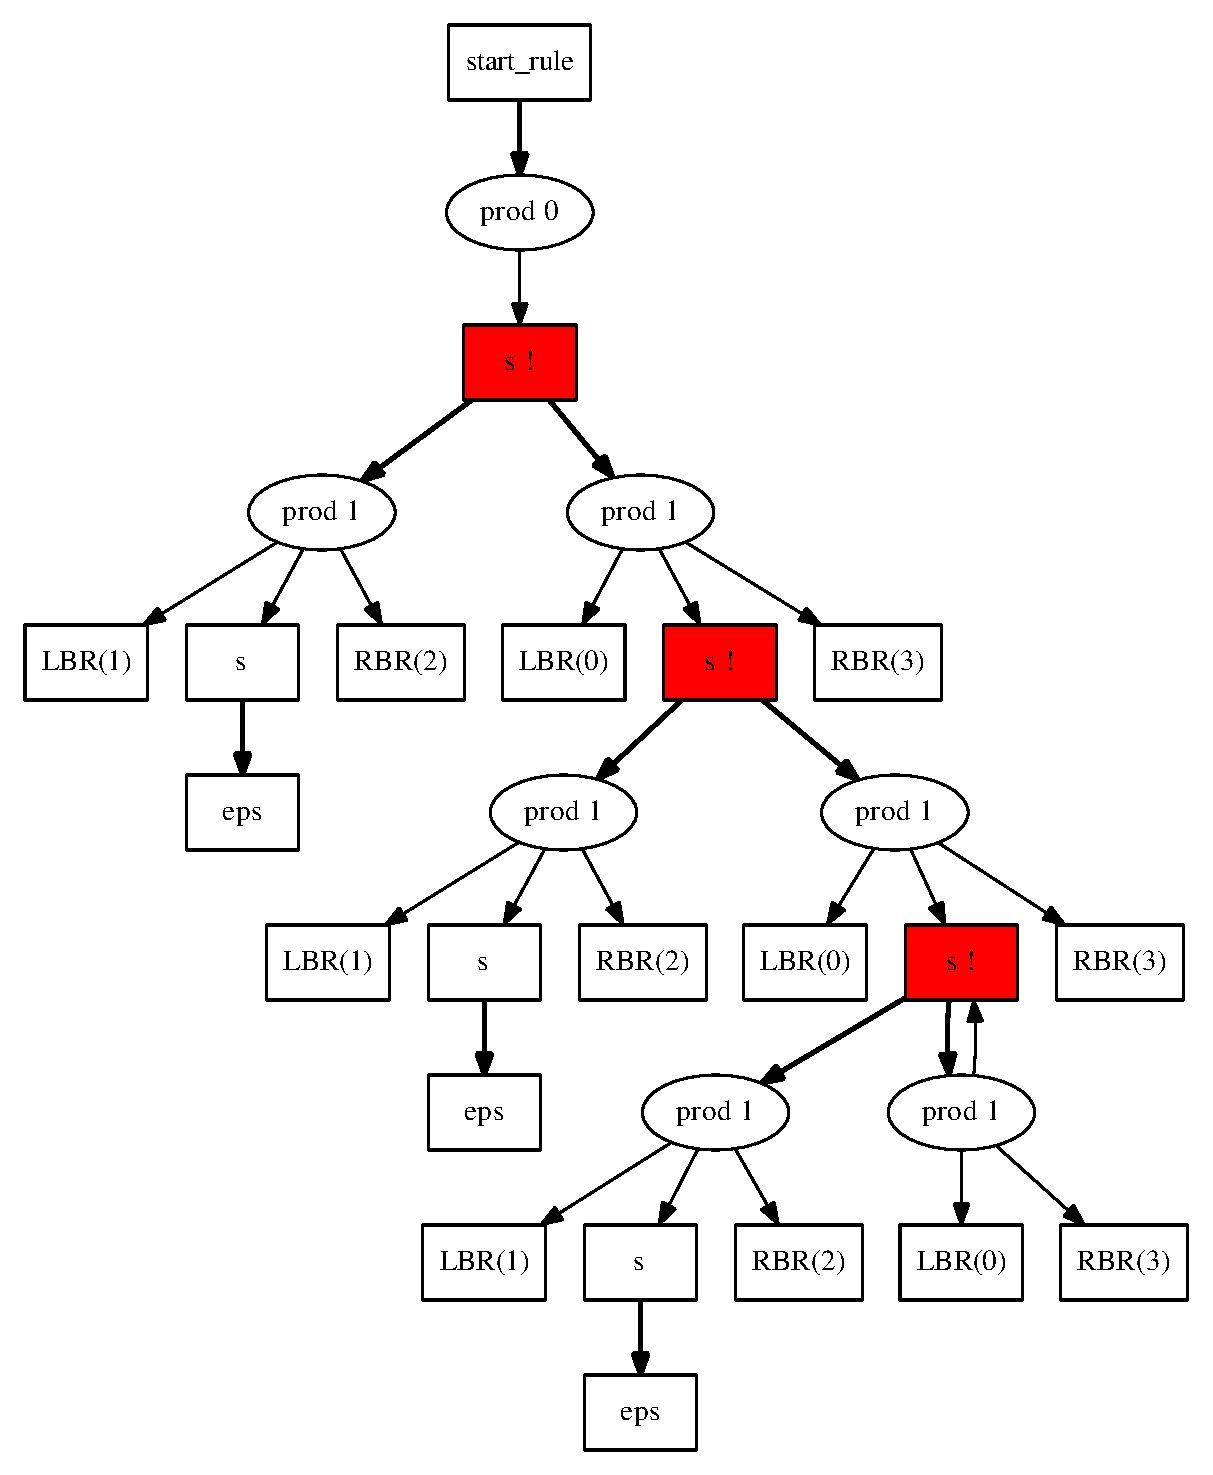
\includegraphics[scale=0.3]{dot/out3.eps}
%    \end{center}
%    \caption{SPPF for input FA presented in figure~\ref{faApprox}}
%    \label{resultSPPF}
%\end{figure}
\pagebreak
\section{\appendixname: RNGLR pseudocode}\label{RNGLRCode}

\begin{algorithm}[]
\begin{algorithmic}[1]
\caption{RNGLR algorithm}
\label{rnglr}
\Function{parse}{$grammar, input$}
  \State{$\mathcal{R} \gets \emptyset$} \Comment{Queue of tuples of GSS vertex, nonterminal, and reduction length}
  \State{$\mathcal{Q} \gets \emptyset$} \Comment{Collection of pairs of GSS vertex and parser state}
  \If{$input = \epsilon$}
    \If{$grammar$ accepts empty input} {report success}
    \Else { report failure}
    \EndIf
  \Else
    \State{\Call{addVertex}{$0, 0, startState$}}
    \ForAll{$i$ in $0..input.Length-1$}
      \State{\Call{reduce}{$i$}}
      \State{\Call{push}{$i$}}
    \EndFor
    \If{$i=input.Length-1$ and there is a vertex in the last level of GSS which state is accepting}
      \State{report success}
    \Else { report failure}
    \EndIf
  \EndIf
\EndFunction
\Function{reduce}{$i$}
  \While{$\mathcal{R}$ is not empty}
    \State{$(v, N, l) \gets \mathcal{R}.Dequeue()$}
    \State{find the set $\mathcal{X}$ of vertices reachable from $v$ along the path of length $(l-1)$}
    \State{or length $0$ if $l=0$}
    \ForAll{$v_{h} = (level_{h}, state_{h})$ in $\mathcal{X}$}
      \State{$state_{t} \gets$ calculate new state by $state_{h}$ and nonterminal $N$}
      \State{\Call{addEdge}{$i, v_{h}, v.level, state_{tail}, (l=0)$}}
    \EndFor
  \EndWhile
\EndFunction
\Function{push}{$i$}
  \State{$\mathcal{Q^{'}} \gets$ copy $\mathcal{Q}$}
  \While{$\mathcal{Q^{'}}$ is not empty}
    \State{$(v, state) \gets \mathcal{Q}.Dequeue()$}
    \State{\Call{addEdge}{$i, v, v.level + 1, state, false$}}
  \EndWhile
\EndFunction
\end{algorithmic}
\end{algorithm}

\begin{algorithm}[]
\begin{algorithmic}[1]
\caption{GSS construction}
\label{RNGLRMain}
\Function{addVertex}{$i, level, state$}
  \If{GSS does not contain vertex $v = (level, state)$}
    \State{add new vertex $v = (level, state)$ to GSS}
    \State{calculate the set of shifts by $v$ and the $input[i+1]$ and add them to $\mathcal{Q}$}
    \State{calculate the set of zero-reductions by $v$ and the $input[i+1]$ and}
    \State{add them to $\mathcal{R}$}
  \EndIf
  \State{\Return{$v$}}
\EndFunction
\Function{addEdge}{$i, v_{h}, level_{t}, state_{t}, isZeroReduction$}
  \State{$v_{t} \gets$ \Call{addVertex}{$i, level_{t}, state_{t}$}}
  \If{GSS does not contain edge from $v_{t}$ to $v_{h}$}
    \State{add new edge from $v_{t}$ to $v_{h}$ to GSS}
    \If{not $isZeroReduction$}
      \State{calculate the set of reductions by $v$ and the $input[i+1]$ and}
      \State{add them to $\mathcal{R}$}
    \EndIf
  \EndIf
\EndFunction
\end{algorithmic}
\end{algorithm}




\end{document}